The Program Tree view allows you to build the robot program in an intuitive graphical way. To code, drag
the available commands from the Command Box and drop them at the desired position in the Program
Tree. The drop position determines whether the commands are siblings or parent and child/children. To
modify command argument, the Options pane [3.4, page 29] will be open automatically (if not, click the
one at the side bar). If you want to move the commands within the program tree, long click the command
and use drag-and-drop. Select the command and click the Cut button to permanently remove it.

The programming of KR1410 is done in the teach pendant for one sheet metal part variant.
It is done so as to test the bending process using the KR1410.
The program tree consists of four sequences which runs in parallel.
Sequence 2 and 3 looks for a signal from PLC for pausing and terminating the current program
respectively. Sequence 4 opens the robotic gripper and unloading station gripper using a push button
for manual operation of the gripper.

\begin{figure}[h]
    \centering
    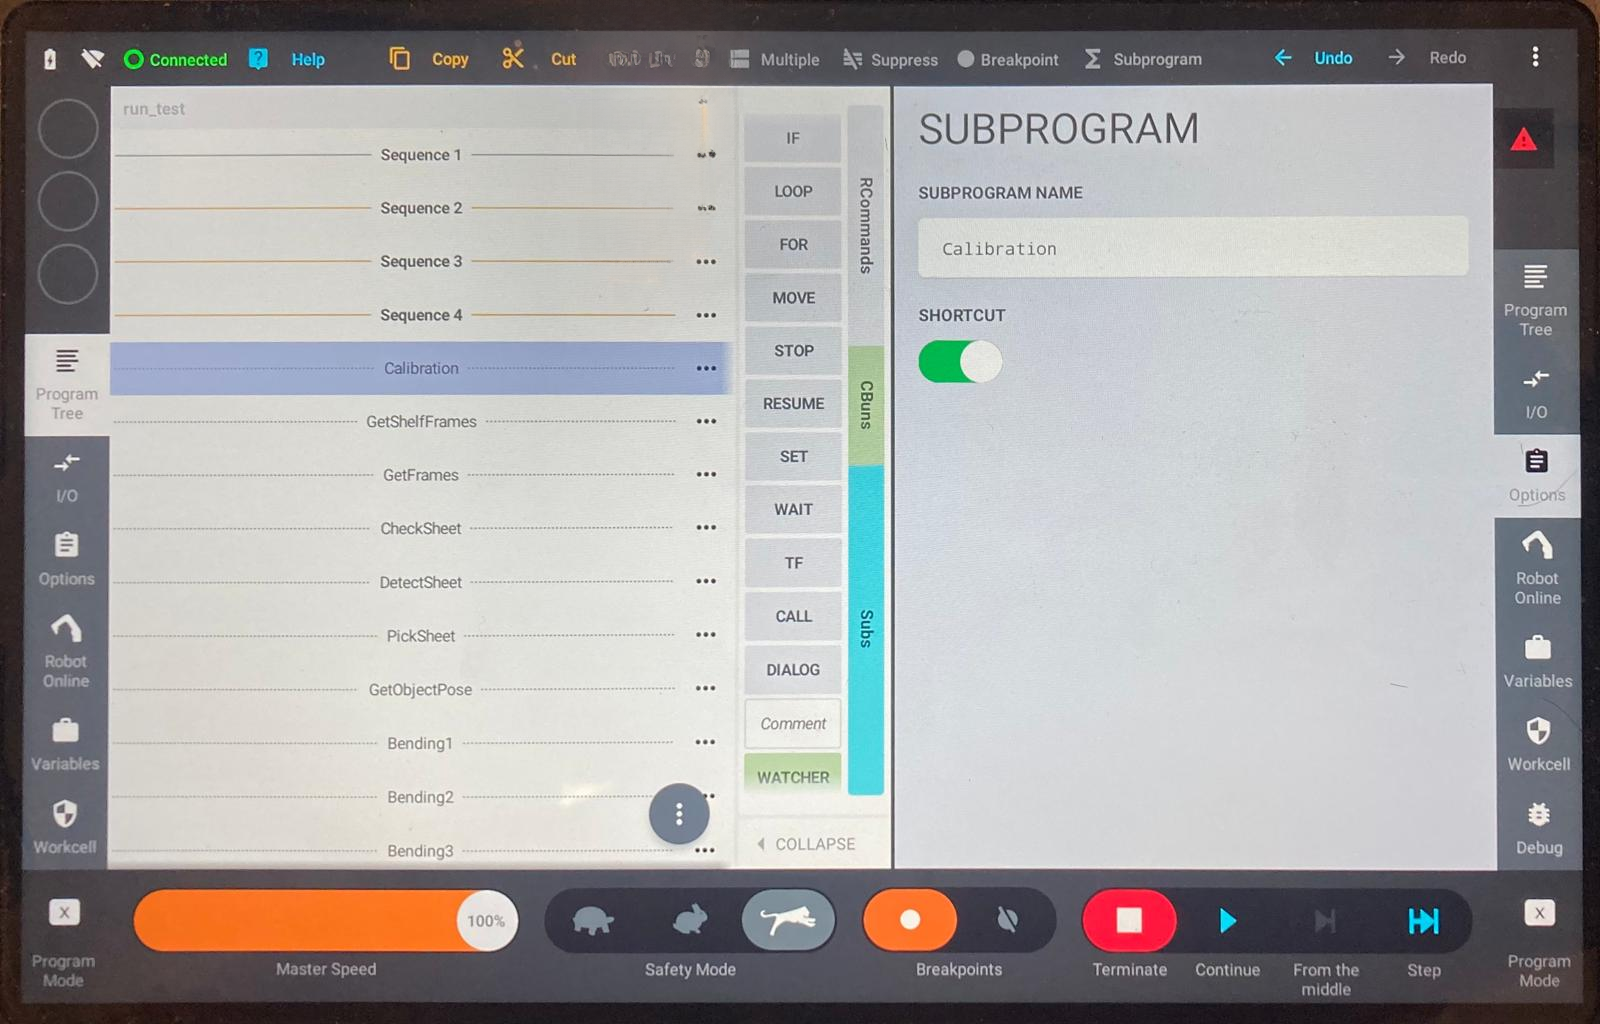
\includegraphics[width=\textwidth]{figures/programtree.png}
    \caption{Programming in teach pendant for a sheet metal part variant}
    \label{fig:programtree}
\end{figure}

Programming is done using a number of subprograms such that a subprogram
can be quickly imported in the sequence and is intuitive to understand as shown in figure \ref{fig:programtree}
Besides normal RCommands like IF, LOOP, FOR, MOVE, WAIT and so on, there are a number of Cbuns modules
from Kassow Robots
imported as well like the IK, FK, WATCHER. IK is used to get the inverse
kinematics from a pose and FK is used to get the forward kinematics
from a joint configuration.
Custom made Cbuns modules for VISOR
are also used for auto-calibration and for getting the pose in the
robot frame of a detected object in the workspace using the robotic camera.

